\documentclass{../../text-style}

\texttitle{Пользовательский интерфейс}

\begin{document}

\maketitle
\thispagestyle{empty}

\section{Введение}

Мы писали по большей части консольные приложения, но понятно, что консольными приложениями пользуются гораздо реже, чем приложениями с графическим (как правило, оконным) интерфейсом. В общем-то, создавать их совсем несложно, и на этой паре будет показано, как это делается. 

В платформе .NET есть целых две библиотеки для разработки пользовательского интерфейса, Windows Forms (WinForms) и Windows Presentation Foundation (WPF). С выходом восьмой винды появилась ещё Microsoft XAML Framework (для разработки так называемых Metro Style приложений, это такие неудобные медленные штуки, работающие без десктопа и окошек), предполагается, что она постепенно заменит WPF, но архитектура и принципы работы у них весьма схожие. Ещё на базе WPF был инструментарий разработки браузерных приложений Silverlight, но он уже несколько лет как не используется, потому что появился HTML 5, который стандартен и покрывает большую часть полезной функциональности Silverlight. WinForms же была первой библиотекой для разработки GUI под .NET, и устарела давно, но поскольку она концептуально гораздо проще WPF, до сих пор активно используется. И на самом деле даже развивается, например, в .NET Framework 4.7 добавилась поддержка экранов с высоким разрешением. Кроме того, WinForms, несмотря на то, что базируется на WinAPI, прекрасно работает под линуксом, а вот с WPF могут возникнуть проблемы. Поэтому, собственно, начнём мы с WinForms, а WPF оставим на третий семестр.

\section{Пример}

Начнём с чего-то вроде <<Hello, world>> на Windows Forms. Обычно приложения рисуют в редакторе форм в Visual Studio, но всё можно делать и прямо из кода. Что особенно полезно, если у вас нет Visual Studio --- Rider вроде как до сих пор редактора форм для WinForms не имеет. Вот, собственно, код:

\begin{minted}{csharp}
public class MyForm : Form {
    public Button button1;

    public MyForm() {
        button1 = new Button();
        button1.Size = new Size(40, 40);
        button1.Location = new Point(30, 30);
        button1.Text = "Click me";
        this.Controls.Add(button1);
        button1.Click += new EventHandler(Button1Click);
    }

    private void Button1Click(object sender, EventArgs e)
    {
        MessageBox.Show("Hello World");
    }

    [STAThread]
    static void Main()
    {
        Application.EnableVisualStyles();
        Application.Run(new MyForm());
    }
}
\end{minted}

Оконное приложение состоит из окон --- наследников класса Form. Где-то, например, в одном из них, есть функция Main, отвечающая за инициализацию и запуск приложения. Обычно она очень короткая, содержит всего две-три строчки, из которых на самом деле обязательна вообще всего одна --- Application.Run, вызов метода, в который надо передать форму, с которой начнётся выполнение. Над Main написан волшебный атрибут [STAThread], это суровое наследие модели потоков ранних версий .NET --- оконные библиотеки все устроены так, что вся работа с элементами пользовательского интерфейса должна выполняться строго из одного потока, этот атрибут говорит компилятору сгенерировать соответствующие инструкции.

Всё интересное происходит на самом деле в конструкторе формы. Там мы создаём кнопку, выставляем её размер, выставляем её координаты относительно окна, выставляем её текст и добавляем как дочерний элемент управления на форму. Элементы управления в WinForms, кстати, называются <<контролы>>. Ещё элементы управления часто называют <<виджетами>>, но это в других библиотеках, например, Qt. 

Дальше мы подписываем обработчик Button1Click на событие Click кнопки. Теперь всякий раз, когда на кнопку кликают (или жмут пробел или Enter, пока она в фокусе), вызывается метод Button1Click, который просто показывает диалоговое окно с текстом.

\section{Класс Control}

Корнем  иерархии классов Windows Forms и центром архитектуры библиотеки является класс Control --- абстракция элемента, из которого строится пользовательский интерфейс. От него наследуется всё, что может быть добавлено на форму --- кнопки, текстовые метки, полосы прокрутки, поля ввода и т.д. Можно создавать свои контролы, наследуясь от этого класса (на самом деле, лучше от UserControl), и они смогут после некоторых усилий вести себя как стандартные. Конкретно Control отвечает за обработку пользовательского ввода (разбирая события из очереди событий, которые ему доставляет контрол-родитель и генерируя правильные события, на которые уже можно подписаться, или вызывая виртуальные методы, которые можно переопределить), и за позицию на экране. В том числе, контрол знает свою длину и ширину, желаемое поведение при растяжении-сжатии по горизонтали-вертикали, которые потом используются в алгоритмах автоматического размещения (лейаутах), чтобы спозиционировать элемент на экране. Но о лейаутах чуть позже.

Вторая важная штука, которую поддерживает Control, это свойства, значения которых наследуются от родителя. В WinForms таких свойств немного --- это Cursor, Font, BackColor, ForeColor и RightToLeft, и нужны они для того, чтобы вся форма выглядела единообразно. Например, можно переопределить цвет фона для формы, и все элементы управления, типа разных панелей, получат свой цвет от формы. Иначе нам пришлось бы вручную переопределять цвет фона для каждого контрола.

Ну и, конечно, у каждого контрола есть список контролов, которые лежат внутри, это свойство Controls. В WinForms это свойство используется только для контролов-контейнеров, типа самой формы, панелей, вкладок и т.д. Наличие этого свойства позволяет организовывать контролы в дерево, в корне которого форма, сыновья которой --- контролы, у которых могут быть свои сыновья и т.д.

\section{Обработка пользовательского ввода}

Реагировать на действия пользователя контролы могут, посылая события, когда происходит что-то интересное. Что-то интересное бывает двух типов --- события клавиатуры и события мыши (на самом деле, есть ещё тачскрин, но он работает в основном как мышь). События с клавиатуры бывают типа KeyDown (клавишу нажали), KeyPress (зафиксировано нажатие), KeyUp (клавишу отпустили), причём при быстром нажатии на клавишу события приходят именно в таком порядке. Если кнопку зажать, то сначала придёт KeyDown, затем несколько раз через равные промежутки времени, задаваемые в настройках операционной системы, KeyPress, затем, когда клавишу таки отпустят, KeyUp. 

Вот небольшой пример обработчика событий от клавиатуры: 

\begin{minted}{csharp}
private void textBox1_KeyDown(object sender, KeyEventArgs e)
{
    if (e.KeyCode == Keys.F1 && (e.Alt || e.Control || e.Shift))
    {
        Help.ShowPopup(textBox1, "Enter your name.", 
            new Point(textBox1.Bottom, textBox1.Right));
    }
}
\end{minted}

Нажатую клавишу можно идентифицировать по свойству KeyCode события, ещё в событие передаётся состояние клавиш-модификаторов Alt, Ctrl и Shift. 

Ещё есть низкоуровневые методы, переопределив которые в своём потомке Control, можно перехватить событие клавиатуры до того, как оно будет диспетчеризовано --- то есть до того, как будут отправлены события. PreProcessMessage делает как раз это, WndProc --- это вообще штука, которая принимает <<сырое>> системное событие из очереди обработки событий для окна и по идее должно диспетчеризовать его дочерним контролам. Но его, конечно, можно переопределить, зачем бы это ни было нужно. Хорошей идеей было бы при переопределении не забыть вызвать метод предка, чтобы не потерять базовой функциональности обработки событий.

События мыши устроены аналогично. При одинарном клике приходят события MouseDown, Click, MouseClick, MouseUp. Обратите внимание, что Click и MouseClick --- это разные вещи. Первое возникает не только когда по контролу кликнули мышкой: нажатие на пробел, когда контрол в фокусе, тоже сойдёт. MouseClick --- это клик конкретно мышкой.

При двойном клике события приходят в порядке MouseDown, Click, MouseClick, MouseUp, MouseDown, DoubleClick, MouseDoubleClick, MouseUp --- обратите внимание, что первый клик в дабл-клике неотличим от обычного клика, а длительность дабл-клика настраивается в свойствах операционной системы, так что делать контролу разную функциональность при реакции на клик и дабл-клик --- обычно плохая идея.

\section{Валидация ввода}

Любая уважающая себя оконная библиотека имеет механизмы, позволяющие легко проверять пользовательский ввод на корректность. Пользователи часто ошибаются, поэтому доверять вводу программа не должна, а должна вежливо сообщать пользователю, что он сделал не так и как это исправить. Для этого в WinForms есть два способа. 

Самый простой, который подходит для  довольно многих случаев и не требует программистских усилий --- использовать контрол MaskedTextBox. Ему можно установить маску --- в каких позициях допустимы цифры, буквы, сколько их  и т.д., и пользователь просто не сможет ввести ничего, что не соответствует маске.

Для более сложных случаев потребуется ловить и обрабатывать событие Validating, которое есть у каждого контрола. В это событие передаётся в качестве аргумента объект класса CancelEventArgs, у которого есть свойство Cancel, которое можно выставить в true, если введённое пользователем значение нам не нравится. Тогда пользователя заставят ввести что-нибудь другое, не дав убрать фокус.

Валидация ввода по умолчанию происходит при потере фокуса ввода. При этом события приходят в такой последовательности:  Leave, Validating, Validated, LostFocus. Validated --- событие, которое шлётся после успешной валидации. Кстати, фокус ввода может иметь ровно один контрол, не только в текущем окне, но во всей операционной системе (на самом деле, в пользовательской сессии), это тот контрол, которому доставляется ввод с клавиатуры. Есть свойство AutoValidate, с помощью которого можно разрешить отдать фокус даже если валидация не прошла. Валидацию можно инициировать не только по потере фокуса, но и вручную --- с помощью методов \mintinline{csharp}{Validate()} и \mintinline{csharp}{ValidateChildren()}.

\section{Data Binding}

Ещё одна штука, которую умеет любая уважающая себя библиотека для создания оконных интерфейсов --- автоматическое связывание с данными. Можно связать какое-нибудь свойство контрола с каким-нибудь полем класса, так, чтобы свойство контрола было всегда равно значению поля, и даже чтобы оно динамически обновлялось, когда меняется свойство в классе и наоборот --- если связать свойство Text у элемента, допускающего пользовательский ввод, с полем, то если пользователь что-то введёт, значение тут же окажется в поле связанного класса (если пройдёт валидацию). Чтобы обеспечить синхронность изменений, надо немного повозиться, так что про это сейчас не будет, но простой пример, показывающий <<однократное>> связывание, вот:

\begin{minted}{csharp}
public partial class Form1 : Form
{
    public string MyText { get; set; } = "Click me";

    public Form1()
    {
        InitializeComponent();
        button1.DataBindings.Add("Text", this, "MyText");
    }
}
\end{minted}

Свойство Text у кнопки будет выставлено в исходное значение свойства MyText у формы, то есть в <<Click me>>, но дальнейшие изменения этого свойства на текст на кнопке никак не повлияют. Тем не менее, есть средства сделать, чтобы влияли, что очень удобно --- интерфейс фактически управляется данными, но это оставляется для самостоятельного изучения.

\section{Best practices}

Вот некоторые общие рекомендации по написанию программ с пользовательским интерфейсом.

\begin{itemize}
    \item Отделяйте логику работы программы от представления. Логику лучше выносить в отдельный класс, а формы делать очень простыми, только вызывая в обработчиках методы класса, отвечающего за логику. Это потом позволит безболезненно поменять представление.
    \item Форма должна адекватно вести себя при ресайзе. Пользуйтесь лейаутами и анкорами (про которые ниже).
    \item Пользовательский интерфейс не должен ломать привычек пользователя. Принято кнопку Ok располагать левее кнопки Cancel, так что если вы сделаете формочку, в которой сначала идёт Cancel, потом Ok, пользователи будут путаться. 
    \item Самые часто используемые элементы интерфейса должны находиться ближе всего к рабочей области. Если требуется пройти через сотню выпадающих меню, чтобы найти нужную штуку, вас проклянут.
    \item Не следует думать, что пользователи будут читать документацию. Интерфейс должен быть интуитивно понятен, все необходимые подсказки и пояснения должны быть видны непосредственно (пользуйтесь всплывающими подсказками или прямо подсказками на форме). Максимально переиспользуйте опыт пользователей – например, если пользователь привык запускать приложения кнопкой F5, то если вы пишете что-то, что может что-то запускать, пусть оно запускает по F5.
\end{itemize}

\section{Демонстрация}

Запускаем студию, Create a new project -> C\# -> All platforms -> Desktop -> Windows Forms App (.NET). Создаётся новый проект, открывается редактор форм с пустой формой. Показываем структуру проекта: под файлом Form1.cs скрываются ещё три файла --- Form1.Designer.cs, Form1.resx, и настоящий Form1.cs. Form1.Designer.cs содержит сгенерированный дизайнером форм код формы, и его нельзя редактировать вручную. Каждый раз, когда вы меняете что-то на форме в редакторе, этот класс перегенерится. Form1.resx содержит ресурсы, используемые на форме, такие как, например, строки, показываемые пользователю. По-хорошему, в коде не должно быть захардкоженых строковых констант и прочей информации, которая может быть зависимой от локали, все такие штуки выносятся в ресурсные файлы, и тогда перевод программы на другой язык сводится просто к замене ресурсов. Мы пока не будем этим заморачиваться. Form1.cs --- это то место, куда, собственно, надо писать код.

Обратите внимание, файлы Form1.Designer.cs и Form1.cs содержат объявление одного и того же класса Form1, объявленного как \mintinline{csharp}{partial}. Собственно, ключевое слово \mintinline{csharp}{partial} говорит компилятору, что в файле содержится только часть объявления класса, и следует поискать ещё файлы, где класс доопределён. \mintinline{csharp}{partial}-ами можно делать любые классы, не только относящиеся к пользовательскому интерфейсу. Должны выполняться следующие требования --- все куски класса должны называться одинаково, быть помеченными \mintinline{csharp}{partial}, быть в одном неймспейсе, иметь неконфликтующие модификаторы видимости. Обычно \mintinline{csharp}{partial}-ы, тем не менее, используются только для сгенерённого кода --- тут они позволяют не заботиться о сохранении пользовательских правок, как в Яве, а просто перегенерить весь файл, когда нужно. Все пользовательские правки будут делаться в другом файле, хотя там и определяется тот же самый класс. Для рукописных классов это неудобно, потому что требуется прыгать по разным файлам, чтобы редактировать класс (плохо с точки зрения, собственно, инкапсуляции: у нас код, делающий одно дело, разбросан по разным местам). После компиляции класс получается один, точно так же, как если бы он был описан в одном файле.

Посмотрим на сгенерённый редактором код Form1.Designer.cs. Сначала идёт объявление поля components, штуки, которая будет содержать в себе всякие компоненты на форме. Дальше перегруженный метод Dispose, который служит для освобождения ресурсов, выделенных объекту. Здесь он просто вызывает Dispose у всех компонентов. Дальше идёт директива \#region --- это просто штука для удобства отображения исходников, код, заключённый в \#region/\#endregion, можно свернуть в редакторе студии (и по умолчанию он будет показываться свёрнутым). Вместо кода будет показываться строка, которая написана после \#region. В обычном коде так тоже можно писать, и иногда (например, в процессе рефакторинга, когда вам надо быстро рассортировать кучу методов по файлу) бывает полезно. Использовать его в уже готовом коде не рекомендуют --- он, как ни странно, ухудшает читаемость, а не улучшает её, скрывая, быть может, интересные куски кода, и заставляя кликать на плюсики. Если у вас такой большой файл, что хочется сделать регионы, имеет смысл разбить его на более мелкие классы и вынести в отдельные файлы.

Дальше идёт метод InitializeComponent, самый интересный на самом деле для нас, поскольку содержит в себе код создания и инициализации всех контролов на форме. Сюда можно смотреть, если требуется сделать что-то вручную в рукописном коде, но вы не знаете как. Менять что-либо здесь бессмысленно. Пока у нас форма пустая, тут ничего особо интересного. this.SuspendLayout(); говорит, что пока не надо пытаться автоматически раскладывать элементы по форме (поскольку они сейчас будут создаваться), в конце вызовется this.ResumeLayout(false);, который скажет библиотеке, что вот теперь правила автоматического размещения элементов (лейаут) можно применять. Между этими вызовами находится код, заполняющий свойства объекта-формы. Теперь посмотрим на Form1.cs и увидим, что единственное содержательное, что там написано, это вызов InitializeComponent в конструкторе. 

Дальше посмотрим на Program.cs. Там используется класс System.Windows.Forms.Application, который позволяет задать глобальные настройки исполнения приложения на WinForms, и содержит тот самый цикл обработки событий, про который шла речь на прошлой паре. EnableVisualStyles даёт возможность использовать стиль операционной системы для отображения окна и контролов на нём, впрочем, это работает только на XP. SetCompatibleTextRenderingDefault задаёт параметры отображения текста на некоторых контролах, и опять-таки, для современных приложений не имеет значения и его лучше не трогать. Метод Run запускает цикл обработки событий и показывает ту форму, которую ему передали.

Теперь собственно как добавлять новые контролы. Кстати, касательно терминологии: в продуктах Майкрософт элементы пользовательского интерфейса принято называть контролами, в некоторых других платформах (например, Qt) --- виджетами. Это одно и то же. Так вот, выбираем пункт меню View -> Toolbox, открывается Toolbox (если он ещё не был открыт), там открываем палитру Common Controls, вытягиваем на форму кнопочку. Сохраняемся, смотрим в Form1.Designer.cs, видим там код создания и инициализации кнопочки. Собственно, тот же самый код можно написать и вручную, прямо в рукописном коде, никакой магии тут нет. 

Вернёмся обратно в дизайнер форм. Открываем окно свойств, если оно ещё не открыто. Иначе View -> Properties Window. Выделяем кнопочку. Самые интересные свойства тут Text (то, что пишется на кнопочке), Name (имя переменной, по которой можно получить доступ к кнопочке из кода). Ещё полезны свойства Visible (показывать/не показывать кнопку на форме), Enabled (кнопочка активна/неактивна), BackColor (цвет кнопки), ForeColor (цвет текста на кнопке), Tag (просто любые данные, которые можно хранить в кнопке, это просто поле типа object, и бывает очень полезно, если мы создаём кнопки динамически, чтобы, например, их различать), TabIndex (задаёт порядок, в котором контролы будут посещены при обходе формы с клавиатуры клавишей Tab), TabStop (будет ли контрол вообще посещён при обходе табом). Ещё есть несколько свойств, относящихся к размещению кнопки на форме и поведению при ресайзе, но про это чуть потом, сначала как делать так, чтобы при нажатии на кнопку что-нибудь происходило.

Для этого применяется отдельная вкладка в окне свойств:

\begin{center}
    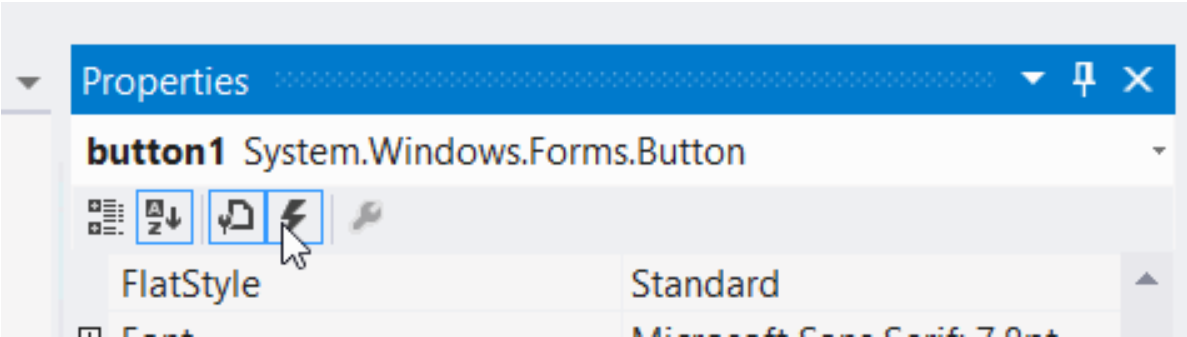
\includegraphics[width=0.5\textwidth]{events.png}
\end{center}

Вообще, сгенерировать обработчик клика на кнопку можно и просто даблкликом на кнопке, но кнопка, как и любой другой контрол, поддерживает ещё кучу всяких событий, каждому из которых тоже можно задать обработчик. Весь список и можно увидеть на вкладке Events. В общем, делаем двойной клик на кнопке, и оказываемся в рукописной части кода класса Form1, в сгенерённом методе-обработчике события клика:

\begin{minted}{csharp}
private void button1_Click(object sender, EventArgs e)
{

}
\end{minted}

Сигнатура должна быть знакома по предыдущему занятию. В Form1.Designer.cs появился соответствующий кусок кода:

\begin{minted}{csharp}
this.button1.Click += new System.EventHandler(this.button1_Click);
\end{minted}

Опять-таки, что тут делается, понятно по предыдущему занятию --- у кнопки есть событие Click, на которое подписывается обработчик \mintinline{csharp}|button1_Click|. Теперь всё-таки сделаем, чтобы что-то происходило, добавив в этот обработчик код, меняющий, скажем, заголовок окна:

\begin{minted}{csharp}
private void button1_Click(object sender, EventArgs e)
{
    this.Text = "Ololo";
}
\end{minted}

\mintinline{csharp}|button1_Click|, хоть и сгенерённое, но всё же плохое имя для контрола, лучше обработчики начинать с On, и следовать общему для всего кода стайлгайду. Просто меняем его имя в Form1.cs на OnButton1Click, жмём Ctrl-. (или кликаем на маленький красный прямоугольник снизу), выбираем нужное действие, он поменяет имя везде, в том числе, и в сгенерённом коде. Точно так же можно и с другими событиями, например, очень легко сделать, чтобы кнопка меняла цвет при наведении на неё мышки. В дизайнере выбираем кнопку, находим её событие MouseEnter во вкладке Events, даблклик по пустому полю с именем метода, пишем обработчик, чтобы получилось как-то так:

\begin{minted}{csharp}
private void button1_MouseEnter(object sender, EventArgs e)
{
    button1.BackColor = Color.Red;
}
\end{minted}

Дальше находим событие MouseLeave и делаем для него обработчик таким:

\begin{minted}{csharp}
private void button1_MouseLeave(object sender, EventArgs e)
{
    button1.BackColor = SystemColors.Control;
}
\end{minted}

Запускаем приложение, проверяем, что всё работает.

Теперь можно поговорить о взаимном расположении контролов на форме. То, что мы сейчас сделали, никуда не годится --- достаточно сжать форму, чтобы понять, почему: кнопка окажется вне отображаемой зоны формы, и по ней будет не кликнуть. Нормальные пользовательские интерфейсы так делать не должны, все элементы управления всегда должны быть доступны, и при этом должны адекватно выглядеть при разных разрешениях экрана. Сама винда вроде как до сих пор имеет окошки системных настроек, которые на нетбуке не лезут на экран, так что даже по кнопке Ok не кликнуть. Для этого используется, во-первых, свойство MinimumSize формы, во-вторых, средства задания положения контролов на форме. 

Первое такое средство --- свойство Anchor контрола. По умолчанию кнопка привязана к левому и верхнему краям формы, так что при изменении размера формы сохранит положение относительно начала координат. Можно привязать кнопку к другим краям формы, если привязать, скажем, к левому и правому, то левая граница кнопки будет привязана к левому краю, а правая --- к правому, так что кнопка будет растягиваться при ресайзе. Если не привязать ни к чему, то кнопка будет стремиться сохранить пропорции расстояний до краёв. Используется всё это в разных ситуациях, например, если у вас есть рабочая область, кнопки слева и кнопки справа, то рабочую область лучше сделать растягивающейся (привязав ко всем краям формы сразу), кнопки слева привязать к левому краю, а кнопки справа --- к правому.

Второе полезное свойство --- Dock, оно позволяет заставить контрол заполнять либо всего контрола-родителя, либо какую-то его часть (верхнюю, левую и т.д.). С ним можно употреблять свойство Margins, задающее отступ в пикселах от границы контрола до границы контрола-родителя (то есть формирующее такую пустую рамку вокруг контрола). Margin-ы можно задавать по отдельности сверху, снизу, справа и слева, и на самом деле это инструмент, который позволяет точно задать положение контрола относительно родителя так, что его будут уважать средства автоматического размещения контрола на форме (лейауты). Поэтому используется даже чаще, чем кажется, хотя полезен и сам по себе, например, принято, чтобы между контролами всегда был какой-то зазор.

Собственно, последний способ управлять положением контролов на форме --- это лейаут. Лейауты можно понимать как алгоритмы размещения контролов. Лейаут спрашивает у контрола, сколько ему места надо обязательно, желательно, максимально, знает свой текущий размер, и из этого вычисляет оптимальные размеры контролов по тому алгоритму, который реализует. Например, FlowLayout просто последовательно выкладывает контролы на форму, не заморачиваясь с размерами и масштабированием. TableLayout представляет форму в виде сетки, где каждый контрол занимает одну или несколько ячеек. При масштабировании ячейки масштабируются пропорционально, и контролы, если им сказано это делать, масштабируются вместе с ними. Лейауты в WinForms используются относительно редко, потому что анкоры --- достаточно выразительный и более простой способ делать масштабируемые формы, но в других библиотеках (например, WPF или Qt) лейауты являются одним из главных средств задания положения элементов. В WinForms лейауты могут быть весьма полезны, если мы динамически создаём контролы во время работы программы, тогда лейаут может положить нам контрол куда надо, какой бы размер ни имела форма.

Рассмотрим подробнее TableLayout. Найти его можно на палитре Toolbox, меню Containers. Выкладываем его на форму, сразу делаем Dock Fill, чтобы заполнить всего родителя (иначе лейаут сам не будет ресайзиться, и толку от него будет немного), задаём ему количество рядов и колонок, и кидаем в одну из получившихся клеток нашу кнопку. У кнопки появляются дополнительные атрибуты Cell, Column, ColumnSpan, Row, RowSpan. ColumnSpan и RowSpan управляют тем, сколько соседних ячеек занимает контрол, так что с их помощью можно делать, например, так:

\begin{center}
    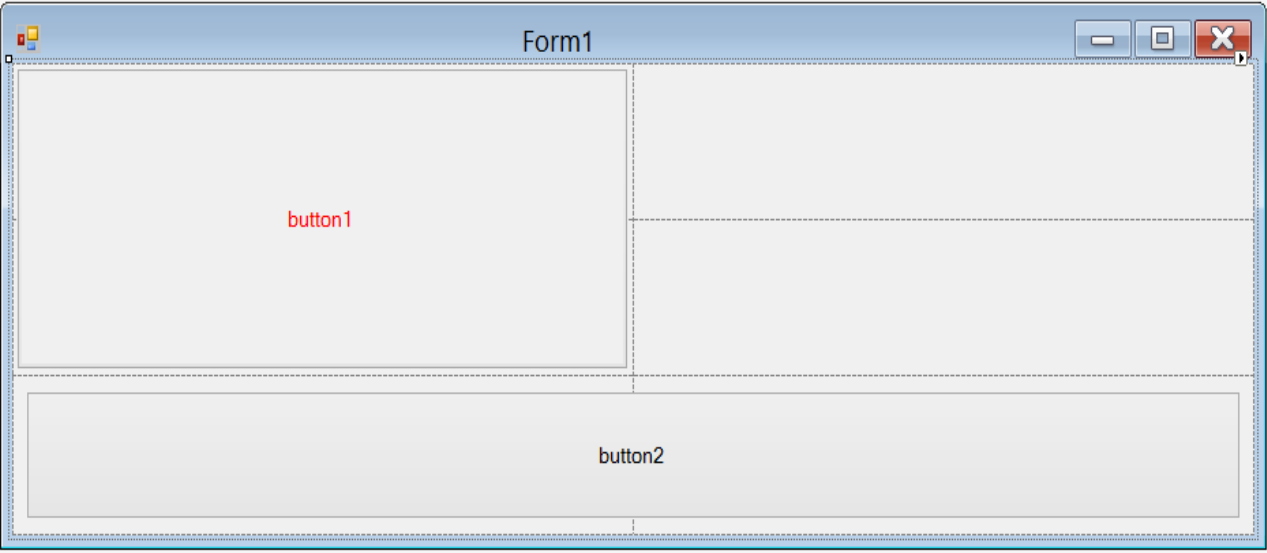
\includegraphics[width=0.7\textwidth]{gridLayout.png}
\end{center}

У самого лейаута тоже есть свойства, наиболее полезные --- Rows и Columns, которые позволяют задать количество и относительные размеры строчек и столбцов сетки.

Дальше можно самим повытаскивать контролы с палитры и посмотреть на то, что они делают. Их довольно много и по ним есть куча документации в интернете, поэтому не будем заморачиваться. Единственное, что, пожалуй, стоит упомянуть в конспекте --- это невизуальные контролы, например, таймер. Таймер просто есть, его можно включить и тогда он будет генерировать события через заданные промежутки времени (один раз или пока его не выключат). На форме он никак не рисуется, но тем не менее, есть в палитре и может редактироваться через редактор свойств, как обычный контрол.

\end{document}
